\documentclass[12pt,letterpaper]{article}
\usepackage[letterpaper,left=0.7in,right=0.7in,top=0.85in,bottom=0.85in,headheight=18pt,headsep=14pt,footskip=0.45in]{geometry}
\usepackage[T1]{fontenc}
\usepackage{newcent}
\usepackage{tikz}
\usepackage{array}
\usepackage{fancyhdr}
\pagestyle{fancy}
\fancyhf{}
\fancyhead[L]{Week 7 / Take-away games / Grades 2--3}
\fancyfoot[L]{Bellingham Math Circle / Week 7}
\fancyfoot[R]{\thepage}
\renewcommand{\headrulewidth}{0.4pt}
\renewcommand{\footrulewidth}{0pt}
\setlength{\parindent}{0pt}
\setlength{\parskip}{0pt}
\hyphenpenalty=10000
\exhyphenpenalty=10000
\setlength{\emergencystretch}{3em}
\newcommand{\prob}[1]{\textbf{Problem #1:}}
\newcommand{\game}[1]{\mbox{\{#1\}}}
\newenvironment{problem}{\par\noindent\begin{minipage}{\linewidth}}{\end{minipage}\par\vspace{0.9cm}}
\begin{document}
In every game in this packet, two players take turns taking counters from a pile. Each problem says how many counters a player may take on a turn. Whoever takes the last counter wins.

\vspace{0.7cm}
\begin{problem}
\prob{1} On each turn, a player takes 1 or 2 counters. For each starting pile in the table, decide whether you would rather go first or second. If you would rather go first, also write how many counters you take on your first turn.
\begin{center}
\renewcommand{\arraystretch}{1.25}
\begin{tabular}{|>{\centering\arraybackslash}m{3.2cm}|>{\centering\arraybackslash}m{4.6cm}|>{\centering\arraybackslash}m{5.4cm}|}
\hline
Starting pile & First or second? & Counters you take first \\ \hline
5\rule[-0.42cm]{0pt}{1.15cm} &  &  \\ \hline
6\rule[-0.42cm]{0pt}{1.15cm} &  &  \\ \hline
7\rule[-0.42cm]{0pt}{1.15cm} &  &  \\ \hline
8\rule[-0.42cm]{0pt}{1.15cm} &  &  \\ \hline
9\rule[-0.42cm]{0pt}{1.15cm} &  &  \\ \hline
10\rule[-0.42cm]{0pt}{1.15cm} &  &  \\ \hline
\end{tabular}
\end{center}
\end{problem}
\begin{problem}
\prob{2} Use the rule from Problem 1. Lee says, ``With 12 counters, I will go second and always win. Whenever you take 1, I take 2, and whenever you take 2, I take 1.'' Mo says, ``With 10 counters, I will go first and take 2, and then I can always win.'' Decide whether each claim is right. If a claim is right, explain why it always works. If it is wrong, show how to beat it.
\vspace{8.0cm}
\end{problem}
\begin{problem}
\prob{3} Now on each turn a player takes 1, 3, or 4 counters. Jo starts with 10 counters and goes first. She takes 3, leaving 7, and says she can now win however the other player plays. Kai starts with 12 counters and goes first. He takes 4, leaving 8, and says the same thing. Decide whether each claim is right. If a claim is right, show how to answer every move the other player can make, all the way to the end of the game. If it is wrong, show how the other player can win.
\vspace{10.5cm}
\end{problem}
\begin{problem}
\prob{4} Use the rule from Problem 3: take 1, 3, or 4 counters on each turn. For each starting pile from 1 to 20, decide whether you would rather go first or second. Shade the box of every pile where you would rather go second. In every other box, write how many counters you take on your first turn.
\vspace{0.2cm}
\begin{center}
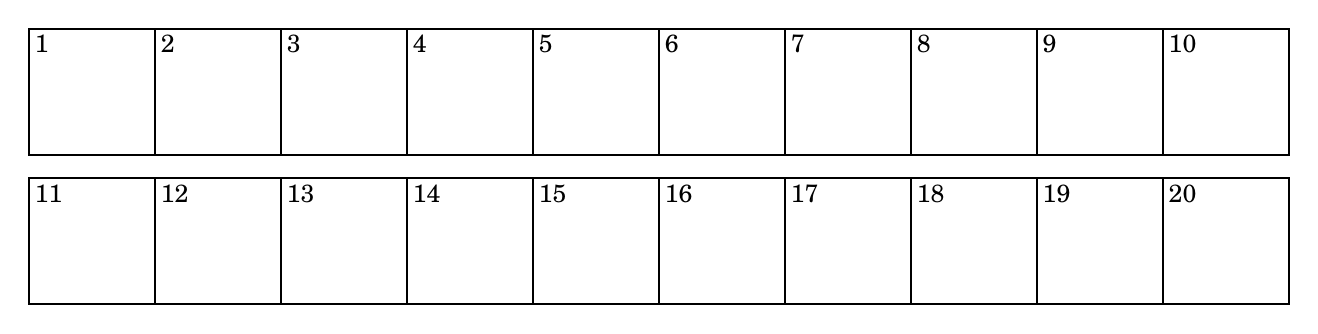
\begin{tikzpicture}
\draw[line width=0.8pt] (0.000,0.000) rectangle (1.600,-1.600);
\node[font=\small,anchor=north west,inner sep=2pt] at (0.000,0.000) {1};
\draw[line width=0.8pt] (1.600,0.000) rectangle (3.200,-1.600);
\node[font=\small,anchor=north west,inner sep=2pt] at (1.600,0.000) {2};
\draw[line width=0.8pt] (3.200,0.000) rectangle (4.800,-1.600);
\node[font=\small,anchor=north west,inner sep=2pt] at (3.200,0.000) {3};
\draw[line width=0.8pt] (4.800,0.000) rectangle (6.400,-1.600);
\node[font=\small,anchor=north west,inner sep=2pt] at (4.800,0.000) {4};
\draw[line width=0.8pt] (6.400,0.000) rectangle (8.000,-1.600);
\node[font=\small,anchor=north west,inner sep=2pt] at (6.400,0.000) {5};
\draw[line width=0.8pt] (8.000,0.000) rectangle (9.600,-1.600);
\node[font=\small,anchor=north west,inner sep=2pt] at (8.000,0.000) {6};
\draw[line width=0.8pt] (9.600,0.000) rectangle (11.200,-1.600);
\node[font=\small,anchor=north west,inner sep=2pt] at (9.600,0.000) {7};
\draw[line width=0.8pt] (11.200,0.000) rectangle (12.800,-1.600);
\node[font=\small,anchor=north west,inner sep=2pt] at (11.200,0.000) {8};
\draw[line width=0.8pt] (12.800,0.000) rectangle (14.400,-1.600);
\node[font=\small,anchor=north west,inner sep=2pt] at (12.800,0.000) {9};
\draw[line width=0.8pt] (14.400,0.000) rectangle (16.000,-1.600);
\node[font=\small,anchor=north west,inner sep=2pt] at (14.400,0.000) {10};
\draw[line width=0.8pt] (0.000,-1.900) rectangle (1.600,-3.500);
\node[font=\small,anchor=north west,inner sep=2pt] at (0.000,-1.900) {11};
\draw[line width=0.8pt] (1.600,-1.900) rectangle (3.200,-3.500);
\node[font=\small,anchor=north west,inner sep=2pt] at (1.600,-1.900) {12};
\draw[line width=0.8pt] (3.200,-1.900) rectangle (4.800,-3.500);
\node[font=\small,anchor=north west,inner sep=2pt] at (3.200,-1.900) {13};
\draw[line width=0.8pt] (4.800,-1.900) rectangle (6.400,-3.500);
\node[font=\small,anchor=north west,inner sep=2pt] at (4.800,-1.900) {14};
\draw[line width=0.8pt] (6.400,-1.900) rectangle (8.000,-3.500);
\node[font=\small,anchor=north west,inner sep=2pt] at (6.400,-1.900) {15};
\draw[line width=0.8pt] (8.000,-1.900) rectangle (9.600,-3.500);
\node[font=\small,anchor=north west,inner sep=2pt] at (8.000,-1.900) {16};
\draw[line width=0.8pt] (9.600,-1.900) rectangle (11.200,-3.500);
\node[font=\small,anchor=north west,inner sep=2pt] at (9.600,-1.900) {17};
\draw[line width=0.8pt] (11.200,-1.900) rectangle (12.800,-3.500);
\node[font=\small,anchor=north west,inner sep=2pt] at (11.200,-1.900) {18};
\draw[line width=0.8pt] (12.800,-1.900) rectangle (14.400,-3.500);
\node[font=\small,anchor=north west,inner sep=2pt] at (12.800,-1.900) {19};
\draw[line width=0.8pt] (14.400,-1.900) rectangle (16.000,-3.500);
\node[font=\small,anchor=north west,inner sep=2pt] at (14.400,-1.900) {20};
\end{tikzpicture}
\end{center}

\end{problem}
\begin{problem}
\prob{5} Keep the rule from Problem 3. For each starting pile in the table, decide whether you would rather go first or second. If you would rather go first, also write how many counters you take on your first turn.
\begin{center}
\renewcommand{\arraystretch}{1.25}
\begin{tabular}{|>{\centering\arraybackslash}m{3.2cm}|>{\centering\arraybackslash}m{4.6cm}|>{\centering\arraybackslash}m{5.4cm}|}
\hline
Starting pile & First or second? & Counters you take first \\ \hline
30\rule[-0.42cm]{0pt}{1.15cm} &  &  \\ \hline
50\rule[-0.42cm]{0pt}{1.15cm} &  &  \\ \hline
61\rule[-0.42cm]{0pt}{1.15cm} &  &  \\ \hline
100\rule[-0.42cm]{0pt}{1.15cm} &  &  \\ \hline
\end{tabular}
\end{center}
\vspace{1.0cm}
\end{problem}
\begin{problem}
\prob{6} Now on each turn a player takes 1, 3, or 5 counters. Shade the box of every starting pile from 1 to 20 where you would rather go second. Explain why the second player can always win from those piles.
\vspace{0.2cm}
\begin{center}
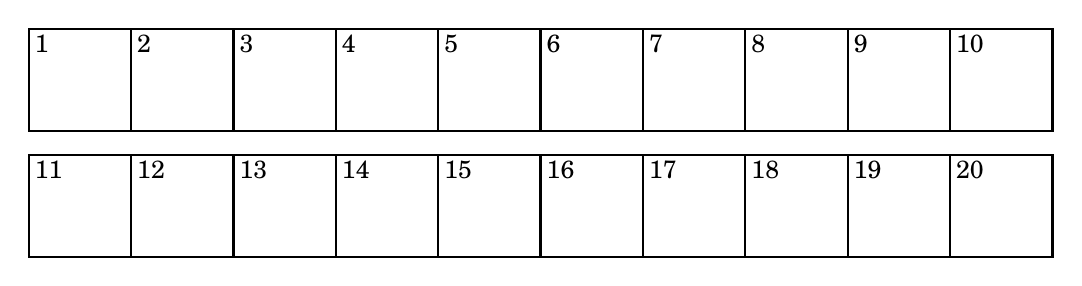
\begin{tikzpicture}
\draw[line width=0.8pt] (0.000,0.000) rectangle (1.300,-1.300);
\node[font=\small,anchor=north west,inner sep=2pt] at (0.000,0.000) {1};
\draw[line width=0.8pt] (1.300,0.000) rectangle (2.600,-1.300);
\node[font=\small,anchor=north west,inner sep=2pt] at (1.300,0.000) {2};
\draw[line width=0.8pt] (2.600,0.000) rectangle (3.900,-1.300);
\node[font=\small,anchor=north west,inner sep=2pt] at (2.600,0.000) {3};
\draw[line width=0.8pt] (3.900,0.000) rectangle (5.200,-1.300);
\node[font=\small,anchor=north west,inner sep=2pt] at (3.900,0.000) {4};
\draw[line width=0.8pt] (5.200,0.000) rectangle (6.500,-1.300);
\node[font=\small,anchor=north west,inner sep=2pt] at (5.200,0.000) {5};
\draw[line width=0.8pt] (6.500,0.000) rectangle (7.800,-1.300);
\node[font=\small,anchor=north west,inner sep=2pt] at (6.500,0.000) {6};
\draw[line width=0.8pt] (7.800,0.000) rectangle (9.100,-1.300);
\node[font=\small,anchor=north west,inner sep=2pt] at (7.800,0.000) {7};
\draw[line width=0.8pt] (9.100,0.000) rectangle (10.400,-1.300);
\node[font=\small,anchor=north west,inner sep=2pt] at (9.100,0.000) {8};
\draw[line width=0.8pt] (10.400,0.000) rectangle (11.700,-1.300);
\node[font=\small,anchor=north west,inner sep=2pt] at (10.400,0.000) {9};
\draw[line width=0.8pt] (11.700,0.000) rectangle (13.000,-1.300);
\node[font=\small,anchor=north west,inner sep=2pt] at (11.700,0.000) {10};
\draw[line width=0.8pt] (0.000,-1.600) rectangle (1.300,-2.900);
\node[font=\small,anchor=north west,inner sep=2pt] at (0.000,-1.600) {11};
\draw[line width=0.8pt] (1.300,-1.600) rectangle (2.600,-2.900);
\node[font=\small,anchor=north west,inner sep=2pt] at (1.300,-1.600) {12};
\draw[line width=0.8pt] (2.600,-1.600) rectangle (3.900,-2.900);
\node[font=\small,anchor=north west,inner sep=2pt] at (2.600,-1.600) {13};
\draw[line width=0.8pt] (3.900,-1.600) rectangle (5.200,-2.900);
\node[font=\small,anchor=north west,inner sep=2pt] at (3.900,-1.600) {14};
\draw[line width=0.8pt] (5.200,-1.600) rectangle (6.500,-2.900);
\node[font=\small,anchor=north west,inner sep=2pt] at (5.200,-1.600) {15};
\draw[line width=0.8pt] (6.500,-1.600) rectangle (7.800,-2.900);
\node[font=\small,anchor=north west,inner sep=2pt] at (6.500,-1.600) {16};
\draw[line width=0.8pt] (7.800,-1.600) rectangle (9.100,-2.900);
\node[font=\small,anchor=north west,inner sep=2pt] at (7.800,-1.600) {17};
\draw[line width=0.8pt] (9.100,-1.600) rectangle (10.400,-2.900);
\node[font=\small,anchor=north west,inner sep=2pt] at (9.100,-1.600) {18};
\draw[line width=0.8pt] (10.400,-1.600) rectangle (11.700,-2.900);
\node[font=\small,anchor=north west,inner sep=2pt] at (10.400,-1.600) {19};
\draw[line width=0.8pt] (11.700,-1.600) rectangle (13.000,-2.900);
\node[font=\small,anchor=north west,inner sep=2pt] at (11.700,-1.600) {20};
\end{tikzpicture}
\end{center}

\vspace{6.0cm}
\end{problem}
\begin{problem}
\prob{7} Now there are two piles. On each turn, a player takes 1 or 2 counters from one of the piles. For each pair of piles below, circle whether you would rather go first or second. When the two piles are the same size, which player can always win? Explain why.
\begin{center}
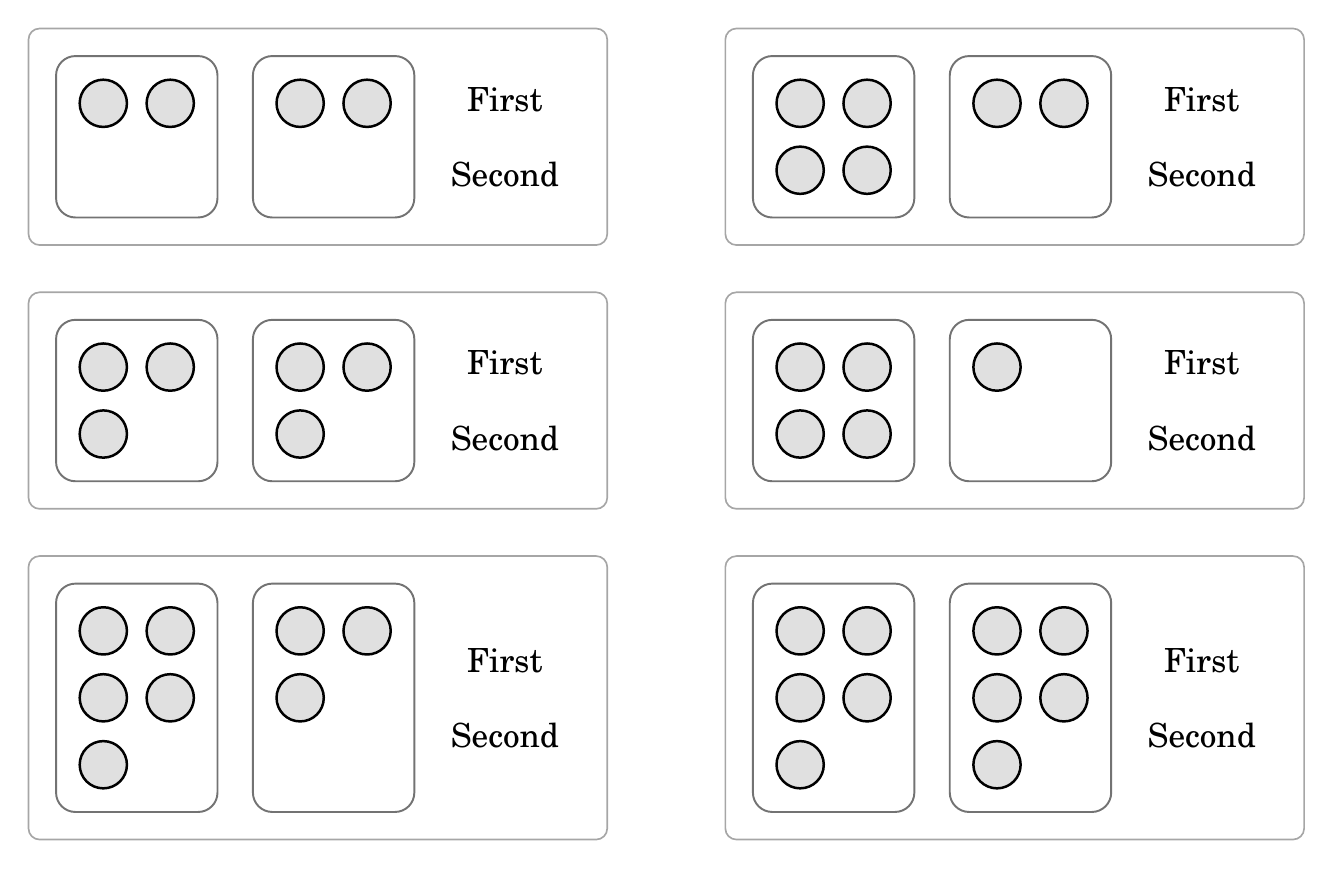
\begin{tikzpicture}
\draw[black!55,line width=0.7pt,rounded corners=7pt] (0.000,0.000) rectangle (2.050,-2.050);
\draw[fill=black!12,line width=0.9pt] (0.600,-0.600) circle (0.3);
\draw[fill=black!12,line width=0.9pt] (1.450,-0.600) circle (0.3);
\draw[black!55,line width=0.7pt,rounded corners=7pt] (2.500,0.000) rectangle (4.550,-2.050);
\draw[fill=black!12,line width=0.9pt] (3.100,-0.600) circle (0.3);
\draw[fill=black!12,line width=0.9pt] (3.950,-0.600) circle (0.3);
\node[font=\large] at (5.700,-0.550) {First};
\node[font=\large] at (5.700,-1.500) {Second};
\draw[black!35,line width=0.6pt,rounded corners=4pt] (-0.350,0.350) rectangle (7.000,-2.400);
\draw[black!55,line width=0.7pt,rounded corners=7pt] (8.850,0.000) rectangle (10.900,-2.050);
\draw[fill=black!12,line width=0.9pt] (9.450,-0.600) circle (0.3);
\draw[fill=black!12,line width=0.9pt] (10.300,-0.600) circle (0.3);
\draw[fill=black!12,line width=0.9pt] (9.450,-1.450) circle (0.3);
\draw[fill=black!12,line width=0.9pt] (10.300,-1.450) circle (0.3);
\draw[black!55,line width=0.7pt,rounded corners=7pt] (11.350,0.000) rectangle (13.400,-2.050);
\draw[fill=black!12,line width=0.9pt] (11.950,-0.600) circle (0.3);
\draw[fill=black!12,line width=0.9pt] (12.800,-0.600) circle (0.3);
\node[font=\large] at (14.550,-0.550) {First};
\node[font=\large] at (14.550,-1.500) {Second};
\draw[black!35,line width=0.6pt,rounded corners=4pt] (8.500,0.350) rectangle (15.850,-2.400);
\draw[black!55,line width=0.7pt,rounded corners=7pt] (0.000,-3.350) rectangle (2.050,-5.400);
\draw[fill=black!12,line width=0.9pt] (0.600,-3.950) circle (0.3);
\draw[fill=black!12,line width=0.9pt] (1.450,-3.950) circle (0.3);
\draw[fill=black!12,line width=0.9pt] (0.600,-4.800) circle (0.3);
\draw[black!55,line width=0.7pt,rounded corners=7pt] (2.500,-3.350) rectangle (4.550,-5.400);
\draw[fill=black!12,line width=0.9pt] (3.100,-3.950) circle (0.3);
\draw[fill=black!12,line width=0.9pt] (3.950,-3.950) circle (0.3);
\draw[fill=black!12,line width=0.9pt] (3.100,-4.800) circle (0.3);
\node[font=\large] at (5.700,-3.900) {First};
\node[font=\large] at (5.700,-4.850) {Second};
\draw[black!35,line width=0.6pt,rounded corners=4pt] (-0.350,-3.000) rectangle (7.000,-5.750);
\draw[black!55,line width=0.7pt,rounded corners=7pt] (8.850,-3.350) rectangle (10.900,-5.400);
\draw[fill=black!12,line width=0.9pt] (9.450,-3.950) circle (0.3);
\draw[fill=black!12,line width=0.9pt] (10.300,-3.950) circle (0.3);
\draw[fill=black!12,line width=0.9pt] (9.450,-4.800) circle (0.3);
\draw[fill=black!12,line width=0.9pt] (10.300,-4.800) circle (0.3);
\draw[black!55,line width=0.7pt,rounded corners=7pt] (11.350,-3.350) rectangle (13.400,-5.400);
\draw[fill=black!12,line width=0.9pt] (11.950,-3.950) circle (0.3);
\node[font=\large] at (14.550,-3.900) {First};
\node[font=\large] at (14.550,-4.850) {Second};
\draw[black!35,line width=0.6pt,rounded corners=4pt] (8.500,-3.000) rectangle (15.850,-5.750);
\draw[black!55,line width=0.7pt,rounded corners=7pt] (0.000,-6.700) rectangle (2.050,-9.600);
\draw[fill=black!12,line width=0.9pt] (0.600,-7.300) circle (0.3);
\draw[fill=black!12,line width=0.9pt] (1.450,-7.300) circle (0.3);
\draw[fill=black!12,line width=0.9pt] (0.600,-8.150) circle (0.3);
\draw[fill=black!12,line width=0.9pt] (1.450,-8.150) circle (0.3);
\draw[fill=black!12,line width=0.9pt] (0.600,-9.000) circle (0.3);
\draw[black!55,line width=0.7pt,rounded corners=7pt] (2.500,-6.700) rectangle (4.550,-9.600);
\draw[fill=black!12,line width=0.9pt] (3.100,-7.300) circle (0.3);
\draw[fill=black!12,line width=0.9pt] (3.950,-7.300) circle (0.3);
\draw[fill=black!12,line width=0.9pt] (3.100,-8.150) circle (0.3);
\node[font=\large] at (5.700,-7.675) {First};
\node[font=\large] at (5.700,-8.625) {Second};
\draw[black!35,line width=0.6pt,rounded corners=4pt] (-0.350,-6.350) rectangle (7.000,-9.950);
\draw[black!55,line width=0.7pt,rounded corners=7pt] (8.850,-6.700) rectangle (10.900,-9.600);
\draw[fill=black!12,line width=0.9pt] (9.450,-7.300) circle (0.3);
\draw[fill=black!12,line width=0.9pt] (10.300,-7.300) circle (0.3);
\draw[fill=black!12,line width=0.9pt] (9.450,-8.150) circle (0.3);
\draw[fill=black!12,line width=0.9pt] (10.300,-8.150) circle (0.3);
\draw[fill=black!12,line width=0.9pt] (9.450,-9.000) circle (0.3);
\draw[black!55,line width=0.7pt,rounded corners=7pt] (11.350,-6.700) rectangle (13.400,-9.600);
\draw[fill=black!12,line width=0.9pt] (11.950,-7.300) circle (0.3);
\draw[fill=black!12,line width=0.9pt] (12.800,-7.300) circle (0.3);
\draw[fill=black!12,line width=0.9pt] (11.950,-8.150) circle (0.3);
\draw[fill=black!12,line width=0.9pt] (12.800,-8.150) circle (0.3);
\draw[fill=black!12,line width=0.9pt] (11.950,-9.000) circle (0.3);
\node[font=\large] at (14.550,-7.675) {First};
\node[font=\large] at (14.550,-8.625) {Second};
\draw[black!35,line width=0.6pt,rounded corners=4pt] (8.500,-6.350) rectangle (15.850,-9.950);
\end{tikzpicture}
\end{center}

\vspace{5.0cm}
\end{problem}
\begin{problem}
\prob{8} Find a rule for how many counters a player may take on a turn, so that you would rather go second exactly when the starting pile is 5, 10, 15, 20, 25, and so on. Then find a different rule that does the same thing.
\vspace{10.0cm}
\end{problem}
\end{document}
